%Plataformas experimentales
\chapter{Sistema de Comunicación}\label{sec:capitulo5}
\thispagestyle{empty}

%\section{Desarrollo del Sistema de Comunicación}
%\subsection{S-Function}
%\subsection{Librería de Socket}
En el presente capítulo se describe el sistema de comunicación implementado en el simulador Dynacar, describiendo la composición de cada bloque, de envío, de recepción y de envío al visor 3D, así como la prueba del mismo a distintas tasas de envío, tanto haciendo uso del visor, como sin hacer uso de este, y de esta forma comprobar si el sistema es válido para las situaciones presentadas.\\

\par No obstante, primero se darán las razones por las cuales se optó por el sistema de comunicación comercial en vez, del vehicular, comparando los estándares de cada uno, y los beneficios que pueda tener uno sobre el otro, en las condiciones presentes en Tecnalia. Posteriormente se tocará el tema de los protocolos de transporte, con el objetivo de conocer cual es el más idóneo para el presente trabajo, para finalmente realizar una descripicón detallada del mensaje a enviar.  


\section{Análisis del Sistema de Comunicación}
Debido a lo complicado y costoso que puede llegar a ser desarrollar un sistema de comunicación vehicular, el presente trabajo propone una alternativa que consiste en emlpear elementos comerciales para realizar las conexiones entre los carros. Sin embargo, como se expuso anteriormente las comunicaciones vehiculares son complejas y requieren de que se cumplan una cierta cantidad de condiciones para efectuarse de manera efectiva, es por esto, que a continuación se compararán ambos sistemas con el fin de demostrar que en ciertos escenarios se puede emular la comunicación vehicular con sistemas comerciales.

\subsection{Sistema de Comunicación Comercial Vs Sistema de Comunicación Vehicular}

Los sistemas de comunicación vehicular hacen uso de los estandares ITS-G5 en Europa. ITS-G5, basan sus capas físicas y MAC en el estándar IEEE 802.11p, descrito en el capítulo 3. A su vez, la norma IEEE 802.11p está realizada bajo la convención IEEE 802.11a, también descrita en el capítulo 3. Ambos estándares emplean la técnica de transmisión OFDM, con la principal diferencia que la IEEE 802.11p hace uso de un ancho de banda de 10 MHz para cada canal, siendo este la mitad que el de IEEE 802.11a. Dicho cambio tiene como finalidad, hacer el sistema más robusto ante el desvanecimiento de las señales, así como aumentar la tolerancia ante los efectos de las señales multitrayecto, que se pueden presentar en los ambientes vehiculares \cite{lin2010comparison}. Las demás diferencias, con respecto a la capa física se pueden encontrar listadas en la tabla \ref{tab:ieeec}.\\   


\begin{table}[htbp]
  \centering
\resizebox{\textwidth}{!}{
    \begin{tabular}{|c|c|c|}
    \toprule

    Parámetro & IEEE 802.11 a & IEEE 802.11 p \\ 
    \midrule

    Tasa de bits & 6,9,12,18,24,36,48,54 & 3, 4, 5, 6, 9, 12, 18 , 24, 27 \\ 
    \midrule

    Tipo de modulación & BPSK, QPSK & BPSK, QPSK \\ 
    \midrule

    Generación del código & 1/2, 2/3, 3/4 & 1/2, 2/3, 3/4  \\ 
    \midrule

    Número de subportadoras & 52    & 52 \\ 
    \midrule

    Duración de los símbolos & 4 us  & 8 us \\ 
    \midrule

    Duración del preámbulo & 16 us & 32 us \\ 
    \midrule

    Espaciado de las subportadoras & 0.3124 MHz & 0.15625 MHz \\ 
    \bottomrule
    \end{tabular}}%
\caption{Comparación entre las capas físicas de los estándares IEEE 802.11p e IEEE 802.11a}
  \label{tab:ieeec}%
\end{table}%

\par Ahora bien, en el caso de la capa MAC ambos stándares emplean el mismo mecanismo de filtrado de mensajes, CSMA/CA, con la diferencia que la IEEE 802.11p, además de usar este mecanismo utiliza el QoS, EDCA, que define cuatro clases distintas de tráfico o categorias de acceso, las cuales poseen diferentes prioridades \cite{milanes2012intelligent}:

 \begin{enumerate}
\item AC\_VO, del inglés \textit{Voice Acces Category}.
\item AC\_VI, del inglés \textit{Video Acces Category}.
\item AC\_BE, del inglés \textit{Best-Effort Acces Category}.
\item AC\_BK, del inglés \textit{Background Acces Ctegory} 
\end{enumerate}

\par Entonces, dependiendo de la prioridad asignada a cada paquete, el mismo será colocado en la cola correspondiente a su categoria de acceso, en el caso de las comunicaciones vehiculares, sí la categoria AC\_VI no es usada, la AC\_VO será priorizada, protegiéndola de cualquier interferencia. Sin embargo, a pesar de esta clasificación, se puede presentar una gran cantidad de pérdida de paquetes, así como un alto delay, al encontrarse bajo circusntancias de tráfico pesado.\\ 

\par En cambio, si se tiene un tráfico ligero y, dependiendo de los mensajes a emplear (emergencias, frenado de emergencia, etc) se puede utilizar la categoria de AC\_VO sin ninguna penalización de delay, y de pérdida de paquetes. Así mismo, para el caso de mensajes periódicos de tipo CAM se tiene el canal de control, CCH (del inlgés, \textit{Control CHanel}), canal donde se pueden enviar y rebicibir los mensajes sin ninguna prioridad asignada, asegurando que se envíen cada 100 ms.\\ 

\par Así pues, el presente trabajo propone un sistema de comunicación comercial donde se tiene un tráfico ligero, más específicamente 2 vehículos, ya sean virtuales o reales, el cual presenta una capa física parecida a la vehicular, es decir, tiene la misma división de canales, con la diferencia de poseer más ancho de banda, lo cual resulta en una menor robustez ante desconexiones abruptas, problema que no se presenta si los individuos están conectados en la misma red.\\
\par En el caso de la capa MAC de los vehículos, se tiene que poseen un variedad de prioridades para reducir el delay de los mensajes y la congestión de conexiones. Sin embargo, sí se emplea el canal CCH, se pueden enviar y recibir mensajes sin tomar en cuenta las prioridades asignadas. Como en el sistema propuesto solo se tienen dos carros, y se estan enviando mensajes del tipo CAM, la comunicación se realiza de forma directa, sin necesidad de que se clasifiquen los mensajes según su prioridad, emulando de esta forma la capa MAC vehicular, en este escenario. El único defecto que se puede presentar es que al no organizar los mensajes, y emplear la misma banda de frecuencia que distintos dispositivos como por ejemplo, los celulares, el sistema es propenso a sufrir interferencias, que puedan generar desconexiones, así como un alto tráfico de mensajes.\\

\par Ya habiendo descrito lo correspondiente a la capa de acceso, ahora se va hablar sobre las capas de transporte, servicios y aplicaciones. En el caso de la capa de trasnporte propuesta se plantean los protocolos UDP o TCP, esto con la asunción de que los vehículos pertenencen a la misma red, por lo que no se necesita nungún tipo de algoritmo de enrutamiento basado en la posición geográfica. Caso similar a la conexión entre vehículos y distintas aplicaciones como el internet.\\

\par Para la capa de servicio, solo se tienen mensajes de tipo CAM, ya que son los necesarios para realizar las maniobras planteadas, a diferencia de los sistemas de comunicación vehicular que poseen tanto mensajes de tipo CAM, como DENM. Para los mensajes CAM, el sistema vehicular plantea una tasa de envío de 100 ms, mientras que en el sistema propuesto se tiene una tasa de envío, entre 1 y 5 ms, rango explicado en el punto 5.2.4. De la misma forma, la tasa de envío en el caso de las comuniaciones V2V es de 10-50 ms.\\

\par Finalmente, en la capa de aplicaciones, al no manejarse mensajes de tipo DENM no se poseen aplicaciones que clasificar, solo las maniobras elavoradas, por lo cual esta capa puede ser descartada a efectos de este trabajo.\\
	            
\subsection{UDP Vs TCP}
\par Para comprender mejor las diferencias existentes entre ambos protocolos, se presenta la tabla \ref{tab:udptcp}, donde se muestra punto por punto las características más reslatantes de ambos protocolos.\\  

% Table generated by Excel2LaTeX from sheet 'Hoja1'
\begin{table}[H]
  \centering
\resizebox{\textwidth}{!}{
    \begin{tabular}{|c|c|c|}
    \toprule
    Característica & TCP   & UDP \\
    \midrule
    Conexión & Es un protocolo orientado a conexiones & \multicolumn{1}{p{16.93em}|}{Es un protocolo que no está orientado a conexiones} \\
    \midrule
    Velocidad de transferencia & \multicolumn{1}{p{18.715em}|}{Debido a su composición presenta una velocidad de transmisión lenta} & \multicolumn{1}{p{16.93em}|}{Debido a su composición posee una velocidad de transmisión rápida} \\
    \midrule
    Uso   & \multicolumn{1}{p{18.715em}|}{Es más orientado a aplicaciones que requieren confiabilidad alta y donde el tiempo de transmisión no es crítico} & \multicolumn{1}{p{16.93em}|}{Es útil en aplicaciones que necesitan trnasmisión rápida.  Es m;as orientado a servidores que reciben una gran cantidad de peticiones de un alto número de clientes} \\
    \midrule
    Orden de los paquetes & \multicolumn{1}{p{18.715em}|}{Reordena paquetes de data en el orden especificado} & \multicolumn{1}{p{16.93em}|}{No posee un orden inherente y los paquetes de data son indeendientes uno del otro. En caso de necesitar un orden, el mismo se tiene que manejar en el nivel de aplicación} \\
    \midrule
    Confiabilidad & \multicolumn{1}{p{18.715em}|}{TCP ofrece garantía absoluta de que la data transferida llegará intacta y en el mismo orden en que fue enviado} & \multicolumn{1}{p{16.93em}|}{No hay garantías de que los paquetes de data lleguen de forma efectiva} \\
    \midrule
    Tamaño de la cabezera & Emplea 20 bits & Emplea 8 bits \\
    \midrule
    Peso  & \multicolumn{1}{p{18.715em}|}{Requiere tres paquetes para establecer una conexión antes de transmitir. TCP maneja confiabilidad y control de congestión } & \multicolumn{1}{p{16.93em}|}{No hay ordenamiento de mensajes ni de conexiones de verificación.} \\
    \midrule
    Verificación de errores & Posee verificación & \multicolumn{1}{p{16.93em}|}{Posee verificación de errores, pero no opciones para recuperar/coregir los mismos} \\
    \midrule
    Reconocimiento & Reconocimiento segmentado & No hace reconocimiento \\
    \midrule
    Verificación en 3 tiempos & SYN, SYN-ACK, ACK & No posee verificación \\
    \bottomrule
    \end{tabular}}%
\caption{Comparación entre los protocolos de transporte TCP y UDP}
  \label{tab:udptcp}%
\end{table}%

\par Repasando la tabla anterior se comprende que el protocolo UDP, es de más utilidad cuando se trata de transmisiones de alta velocidad. Esto se debe a que UDP no está orientado a conexiones, por lo que no posee reconocimiento de paquetes, verificiación de tres tiempos, ni orden inherente en los paquetes, lo que a su vez produce que los mesajes se puedan perder en el camino o lleguen de forma desordenada, mientras que el protocolo TCP  está orientado a garantizar que las conexiones se realicen efectivamente, por lo que si ejecutan reconocimiento, verificación en tres tiempos y ordena los paquetes, con el defecto de que la velocidad de envío de paquetes es muy lenta.\\
\par Entonces, tomando en cuenta estas características, se escogió el protocolo UDP, ya que a pesar de que se pueda correr el riesgo de pérdida de paquetes, la velocidad de envío que proporciona es mayor que la de TCP, por lo que garantiza que los mensajes se puedan enviar dentro de los márgenes que exigen los sistemas de comunicación vehicular. Además al estar orientado a las conexiones, TCP tiene que pasar por todo el proceso de enlace cada vez que se conecten los dispositivos, lo que implica que, si se llega a perder la comunicación, la reconexión de los vehículos no se realiza de forma automática, acción que dificulta un enlace efectivo entre carros. Dicha característica es frecuente en las VANET's por lo cual no se puede correr el riesgo de este problema. Este conflicto no se presenta con el protocolo UDP, que no posee verificiación de conexión, por lo que envía y recibe conestantemente los paquetes sin importar si el enlace está presente.\\

\subsection{Descripción del Mensaje a Enviar}
Para la elección del mensaje se usó como guía el expuesto por la sociedad de ingenieros de automoción, SAE (del inglés,\textit{ Society of Automotive Engineers}), en su documento SAE J2735 \cite{park2011integrated} (Figura \ref{fig:men1}).\\

\begin{figure}[!h]
	\centering
		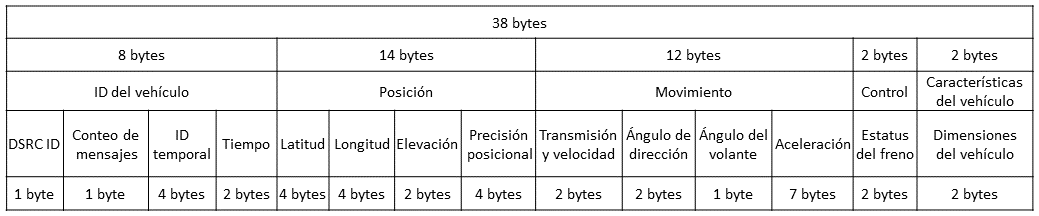
\includegraphics[scale=0.6]{Imagenes/men1}
		\caption{Mensaje propuesto por la SAE}
		\label{fig:men1}
	\end{figure}	
\par Ell mensaje que se propone es una versión más simplificada del mostrado anteriormente, tomando las siguientes consideraciones:

\begin{itemize}
\item Campo de ID del vehículo: debido a que solo se está trabajando con dos vehículos bajo una misma red, no se necesita ningún tipo de identificación por parte de ambos, es por esto que se remueve completamente el campo, a excepción del tiempo, el cual es enviado en segundos.
\item Campo de posición: debido a que el simulador trabaja es con las coordenadas X e Y, se sustituyeron la latitud y la longitud por estas, además al no trabajarse con la elevación, la misma fue eliminada, así como también la precisión posicional.
\item Campo de movimiento: en este campo solo se removió la transmisión, debido a que no es empleada.
\item Control: no posee ningún cambio.
\item Características del vehículo: debido a que los vehículos usados poseen los mismos atributos físicos, se removió este campo, ya que no hay necesidad de enviar datos que ya conocidos por ambos carros.
\end{itemize}
\par Además de estos cambios, debido a que en simulink se trabaja con variables del tipo double, los datos a enviar poseen una longitud de 8 bytes. Así pues, el mensaje empleado puede ser visto en la figura \ref{fig:mem2}.

\begin{figure}[!h]
	\centering
		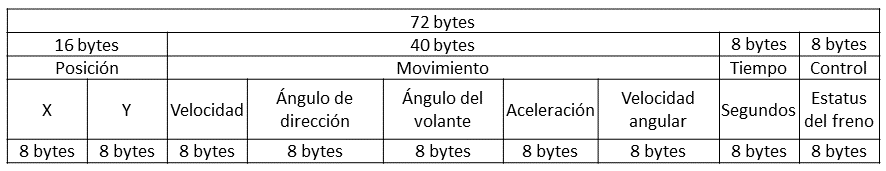
\includegraphics[scale=0.6]{Imagenes/mem2}
		\caption{Mensaje propuesto}
		\label{fig:mem2}
	\end{figure}	  

\section{Implementación en Dynacar}
Como se comentó en secciones anteriores, el sistema de comunicación se programó empleando las S-function, conjunto a la libreria de sockets de Windows, todo esto en los entornos de MATLAB y Simulink. Así pues, se diseñaron tres bloques, uno para enviar la data a otros vehículos, uno para recibir la data de otros vehículos y por último uno para envíar la data del vehículo con el cual que es está realizando la comunicación al Visor 3D de Dynacar. 
\subsection{Módulo de Envío}
Es el módulo encargado de realizar el envío de la data (Figura \ref{fig:send}), posee como entradas:
\begin{itemize}
\item Posición X, Y, ángulo de dirección y velocidad.
\item Ángulo del volante.
\item Tiempo
\item Velocidad angular.
\item Acelerador y Freno.
\end{itemize}

\begin{figure}[!h]
 \centering
  \subfloat[Bloque de envío]{
   \label{fig:a}
    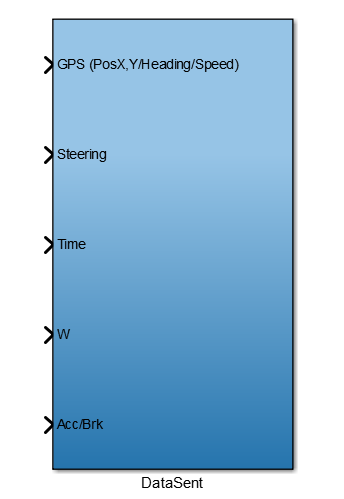
\includegraphics[scale=0.3]{Imagenes/send}}
  \subfloat[Interior del Bloque de envío]{
   \label{fig:v}
    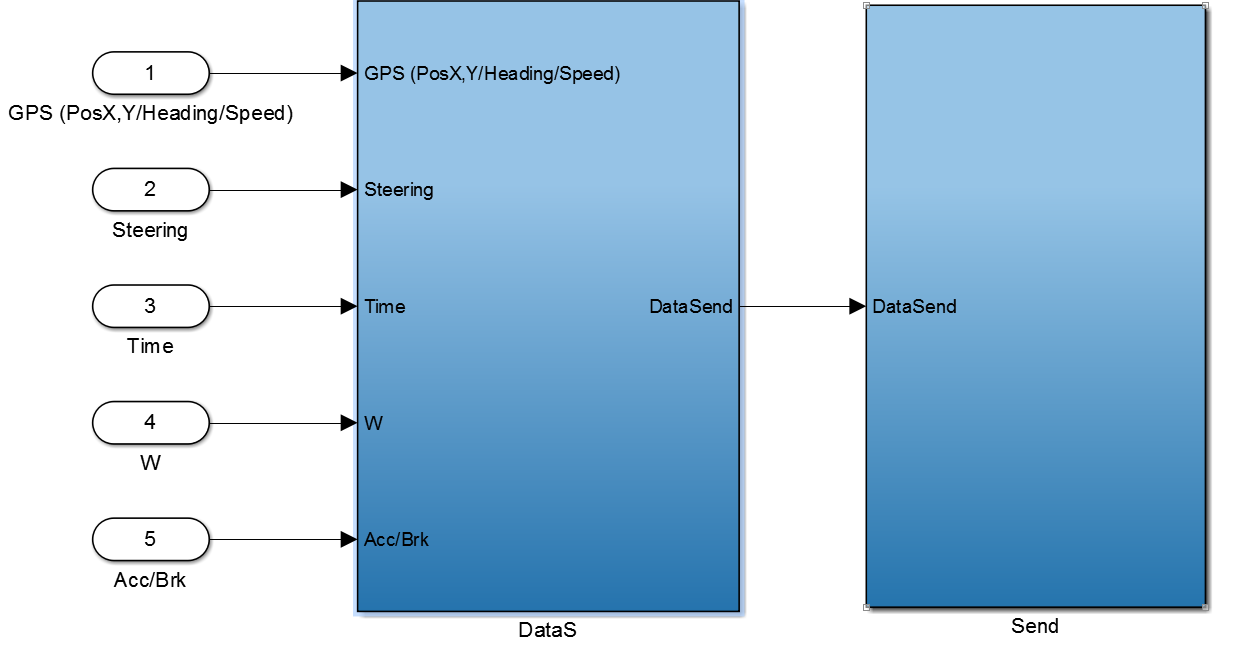
\includegraphics[scale=0.2]{Imagenes/send1}}\\
  \subfloat[Sub-modelo Send]{
   \label{fig:x}
    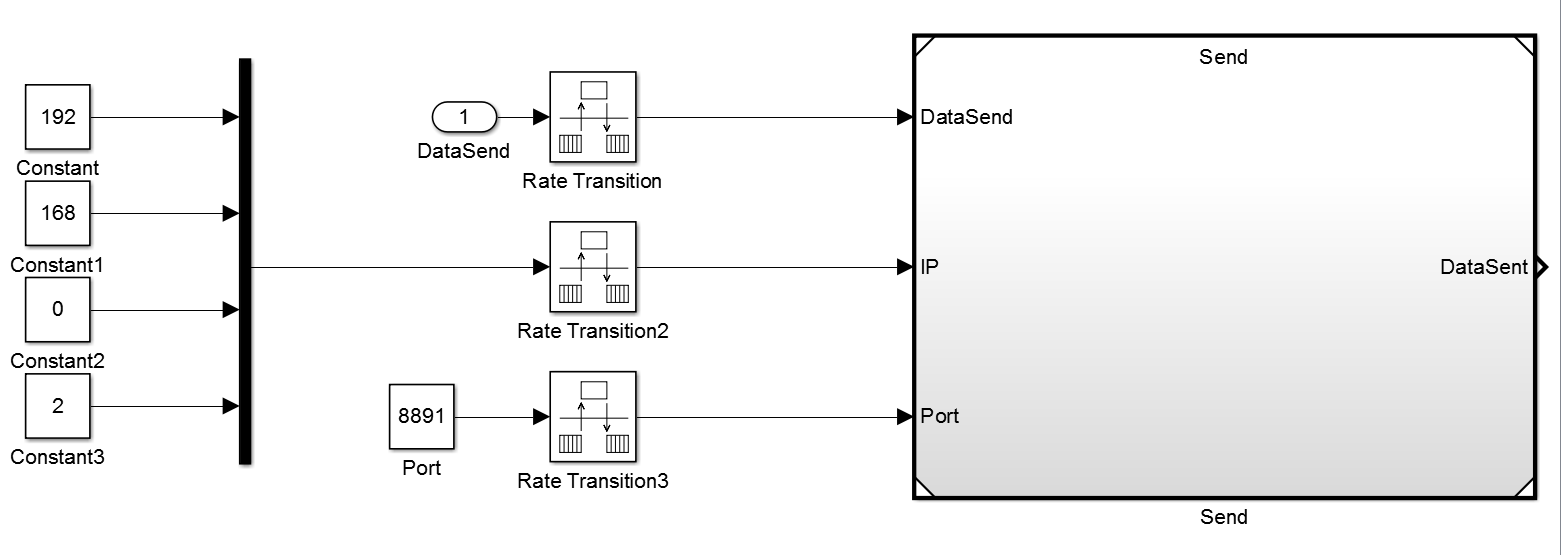
\includegraphics[scale=0.2]{Imagenes/send2}}
 \caption{Estructura del módulo de send}
 \label{fig:send}
\end{figure}

\par Dentro del mismo se encuentra la S-function realizada, que además de recibir los datos a enviar, recibe el IP y el puerto con el cual se va a efectuar la comunicación, datos necesarios para enlazar la computadora con su destino. Una vez activo, dicho bloque siempre estará enviando información, a pesar de que se pueda perder la conexión. Cabe resaltar, que para variar la tasa de envío, se empleó la modalidad de sub-modelos de Simulink, donde en un diagrama principal, se pueden tener bloques secundarios que funcionen a distintos tiempos de muestreo, lo que permite cambiar la tasa, independientemente del esquema principal.          
\subsection{Módulo de Recepción}
Es el bloque encargado de recibir la data proveniente del otro vehículo (Figura \ref{fig:rec}), posee como salidas:

\begin{itemize}
\item Posición X, Y y ángulo de dirección.
\item Velocidad
\item Ángulo del volante.
\item Aceleración.
\item Tiempo.
\item Velocidad angular.
\item Freno.
\end{itemize}

\par Dentro del mismo se encuentra la S-function realizada, que recibe como parámetro, el puerto por el cual se va a obtener la data. Debido a la configuración de los sockets, los mismos están programados para bloquearse hasta recibir información, lo cual perjudica el comportamiento del programa, es por esto que los sockets se configuraron de tal forma que el tiempo de espera sea mayor o igual al tiempo de muestreo del diagrama de simulink, siendo este 1 ms para el simulador y 10 ms para los vehículos. Cabe resaltar, que de la misma forma que para el bloque de envío, se se varía la tasa de recepción a través de un sub-modelo.   

\begin{figure}[!h]
 \centering
  \subfloat[Bloque de recepción]{
   \label{fig:a}
    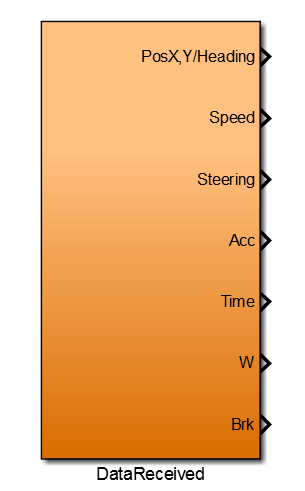
\includegraphics[scale=0.3]{Imagenes/rec2}}
  \subfloat[Interior del Bloque de recepción]{
   \label{fig:v}
    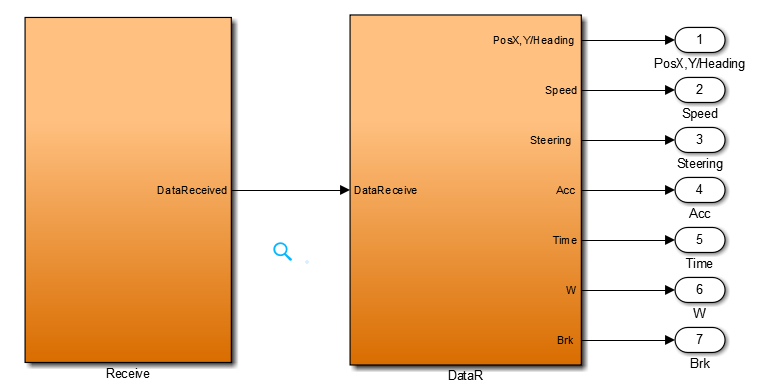
\includegraphics[scale=0.3]{Imagenes/rec1}}\\
  \subfloat[Sub-modelo Receive]{
   \label{fig:x}
    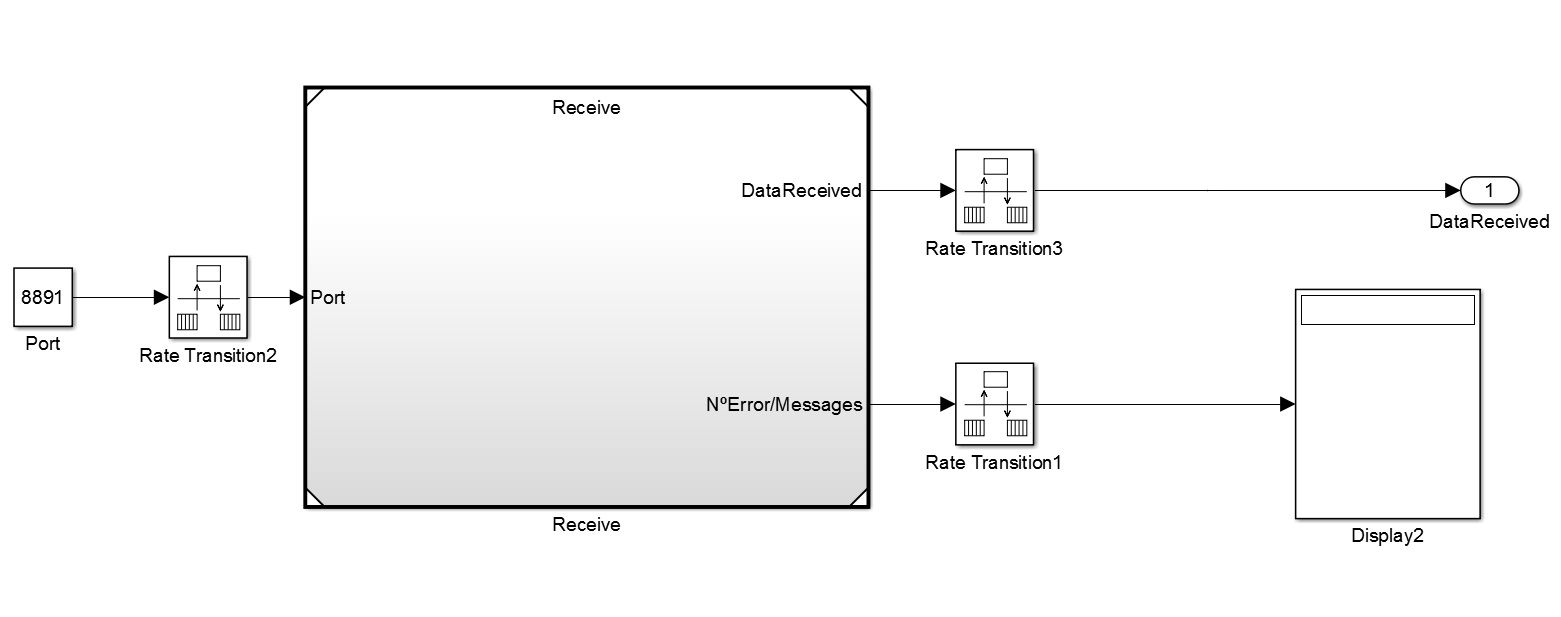
\includegraphics[scale=0.2]{Imagenes/rec3}}
 \caption{Estructura del módulo de recepción}
 \label{fig:rec}
\end{figure}

\subsection{Módulo de Envío al Visor 3D}
Es el módulo encargado de realizar el envío de la data proveniente del vehículo con el cual se está realizando la comunicación (Figura \ref{fig:send}), posee como entradas:

\begin{itemize}
\item Posición X, Y y el ángulo de dirección.
\end{itemize}
\begin{figure}[!h]
 \centering
  \subfloat[Bloque de envío al Visor 3D]{
   \label{fig:a}
    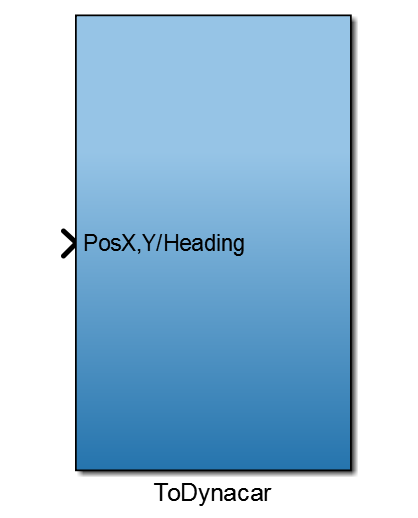
\includegraphics[scale=0.3]{Imagenes/sendtd}}
  \subfloat[Interior del Bloque de envío al Visor 3D]{
   \label{fig:v}
    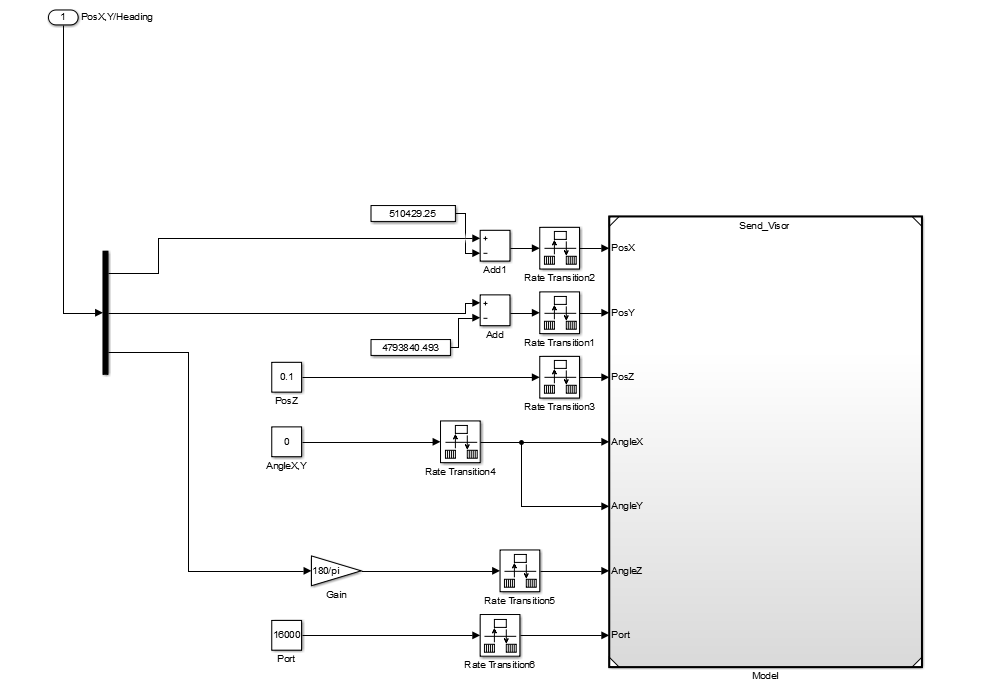
\includegraphics[scale=0.3]{Imagenes/sendtd1}}\\
 \caption{Modelo de envío de información al Visor 3D}
 \label{fig:rec}
\end{figure}

\par Dentro del mismo se encuentra la S-function realizada, que recibe como entrada, el puerto al cual se va a enviar la información, debido a que es una comunicación interna, entre Simulink y el Visor 3D la IP se fija en 127.0.0.1, la cual es empleada cuando se quiere enviar información localmente, o recibir información de cualquier dispositivo. Además el bloque recibe los ángulos con respecto a los otros ejes y la posición en Z, valores que se establecen como 0, debido que no se presenta ningún tipo de movimiento en estos ejes. De la misma forma que para los bloques anterior se realizó un sub-modelo, con el cual se varia la tasa de envío, dicha tasa se fijó en 5 ms para minimizar el coste computacional, y no presentar efectos de retraso con respecto al esquema principal de Dynacar.  

\subsection{Prueba del Sistema de Comunicación a Distintas Tasas de Envío}

Debido a la probablidad de pérdida de paquetes que se puede presentar al utilizar el protocolo UDP, se procede a observar el comportamiento de uno de los módulo que emplee los datos provenientes del vehículo con el cual se está conectado, más específicamente se observa el módulo del ACC, y como responde el controlador ante los mensajes perdidos y las diferentes tasas de envío.\\
 \par Más concretamente, se realizaron 6 pruebas por cada tasa de envío considerada, siendo estas 1 ms, 5 ms, 10 ms, 15, ms 25 ms, 50 ms y 100 ms, de las cuales se reportó la cantidad total de mensajes envíados y mensajes perdidos. Cabe destacar que se este conjunto de pruebas se hicieron tomando en cuenta los efectos que pueda producir el visor 3D.
\subsubsection{Pruebas sin el Visor 3D}  

\begin{itemize}
\item 1 ms
\begin{figure}[H]
	\centering
		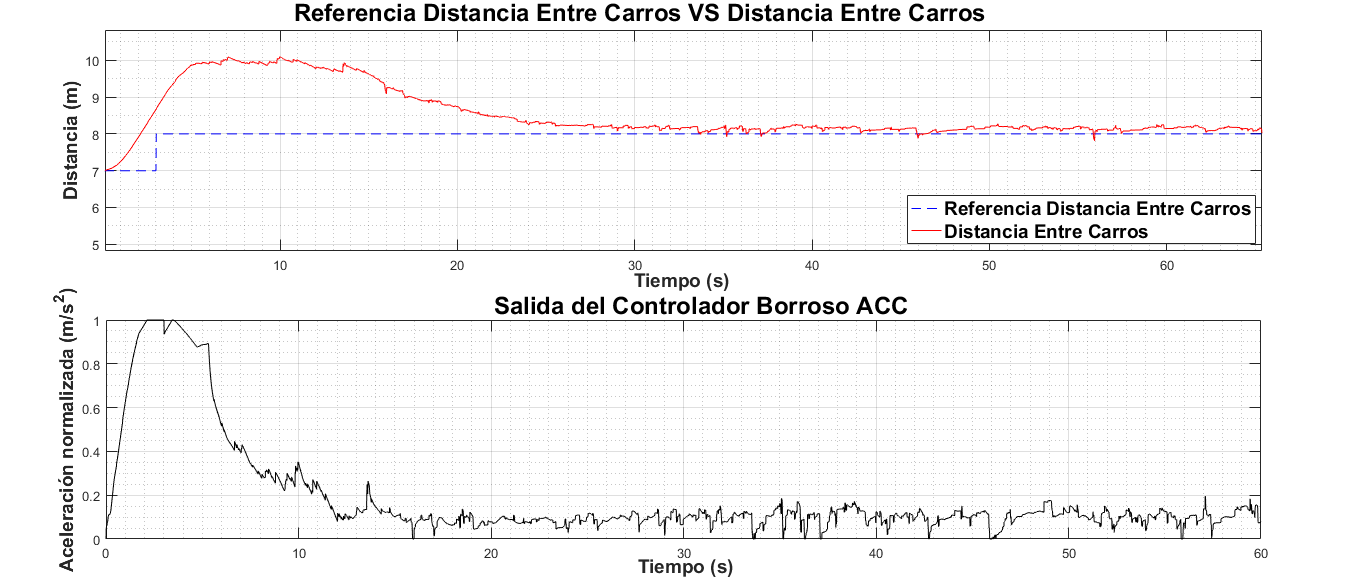
\includegraphics[scale=0.49]{Imagenes/1cv}
		\caption{Gráfica del comportamiento del controlador con una tasa de envío de 1 ms}
		\label{fig:sv1}
\end{figure}
\item 5 ms\\
\begin{figure}[H]
	\centering
		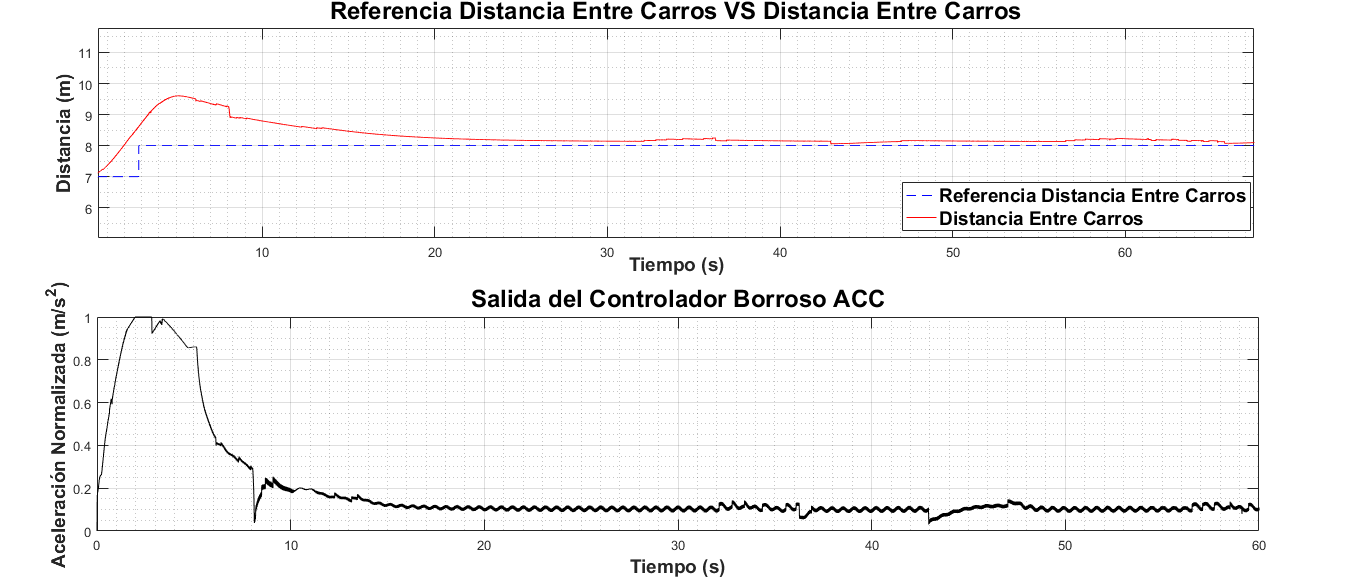
\includegraphics[scale=0.49]{Imagenes/5cv}
		\caption{Gráfica del comportamiento del controlador con una tasa de envío de 5 ms}
		\label{fig:sv5}
\end{figure}	
\item 10 ms
\begin{figure}[H]
	\centering
		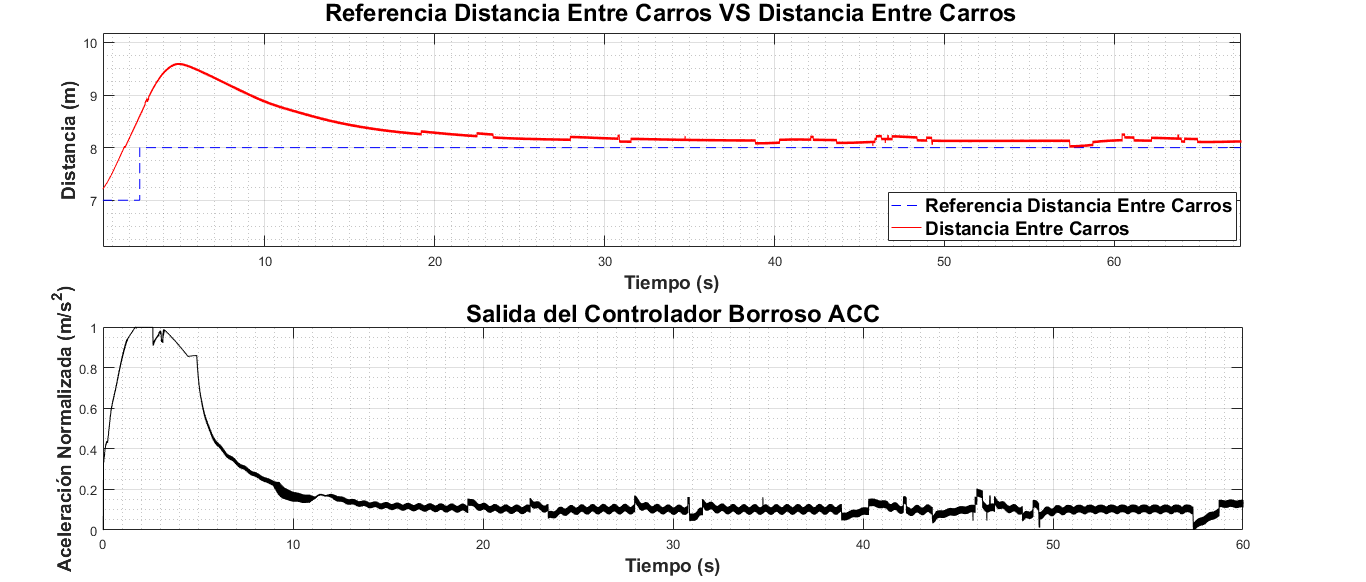
\includegraphics[scale=0.495]{Imagenes/10sv}
		\caption{Gráfica del comportamiento del controlador con una tasa de envío de 10 ms}
		\label{fig:sv10}
\end{figure}	
\item 15 ms
\begin{figure}[H]
	\centering
		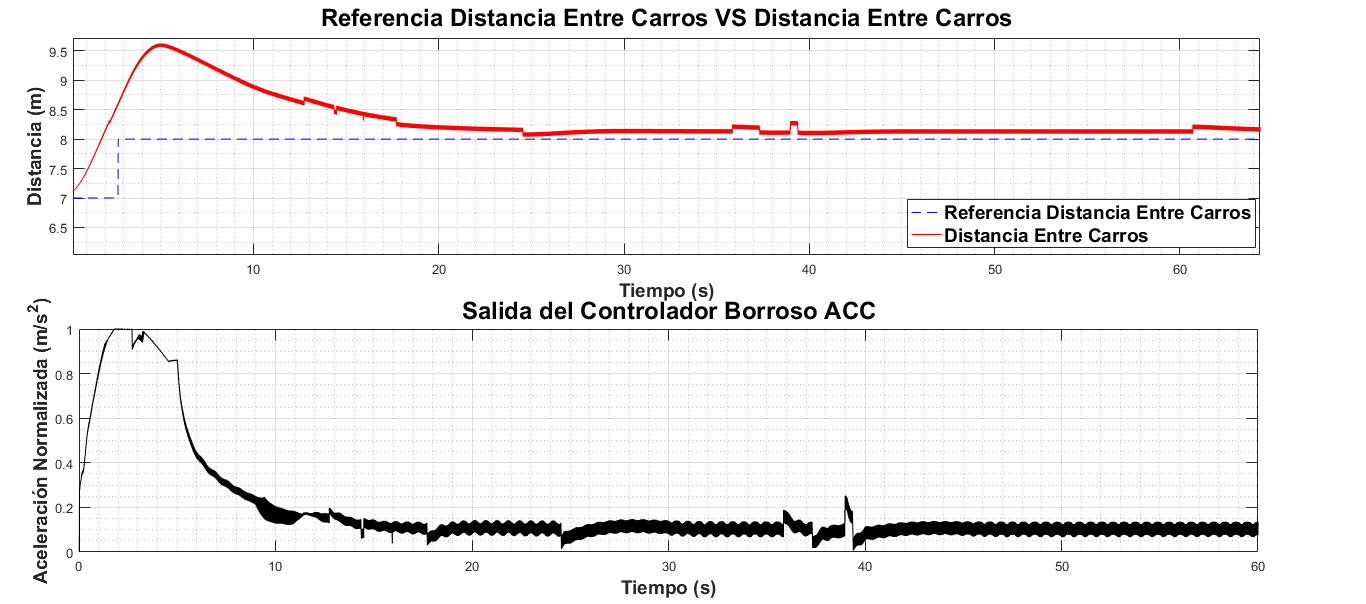
\includegraphics[scale=0.49]{Imagenes/15sv}
		\caption{Gráfica del comportamiento del controlador con una tasa de envío de 15 ms}
		\label{fig:sv15}
\end{figure}	
\item 25 ms
\begin{figure}[H]
	\centering
		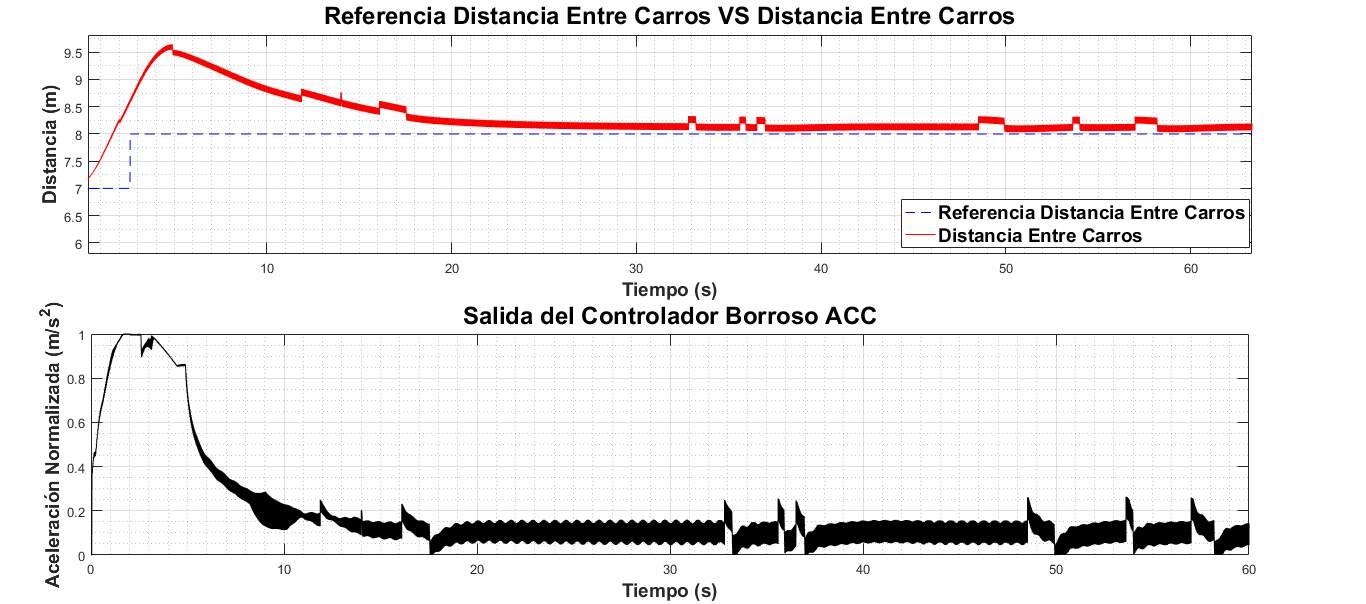
\includegraphics[scale=0.49]{Imagenes/25sv}
		\caption{Gráfica del comportamiento del controlador con una tasa de envío de 25 ms}
		\label{fig:sv25}
\end{figure}	
\item 50 ms
\begin{figure}[H]
	\centering
		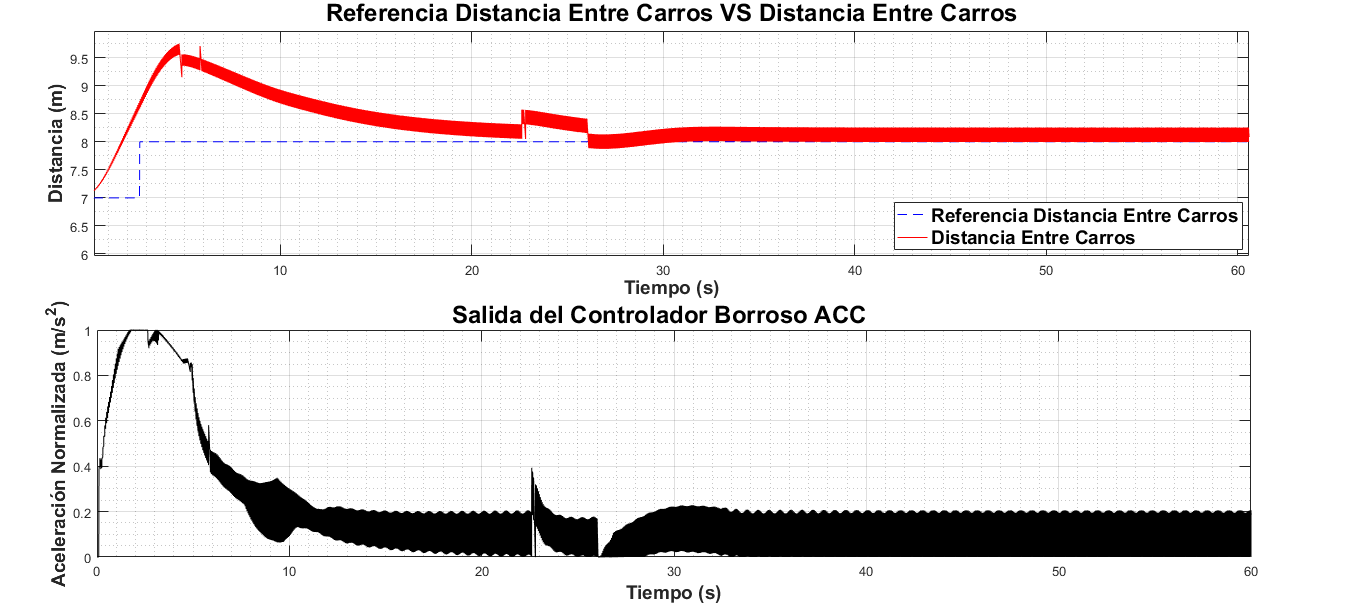
\includegraphics[scale=0.49]{Imagenes/50cv}
		\caption{Gráfica del comportamiento del controlador con una tasa de envío de 50 ms}
		\label{fig:sv50}
\end{figure}	

\item 100 ms
\begin{figure}[H]
	\centering
		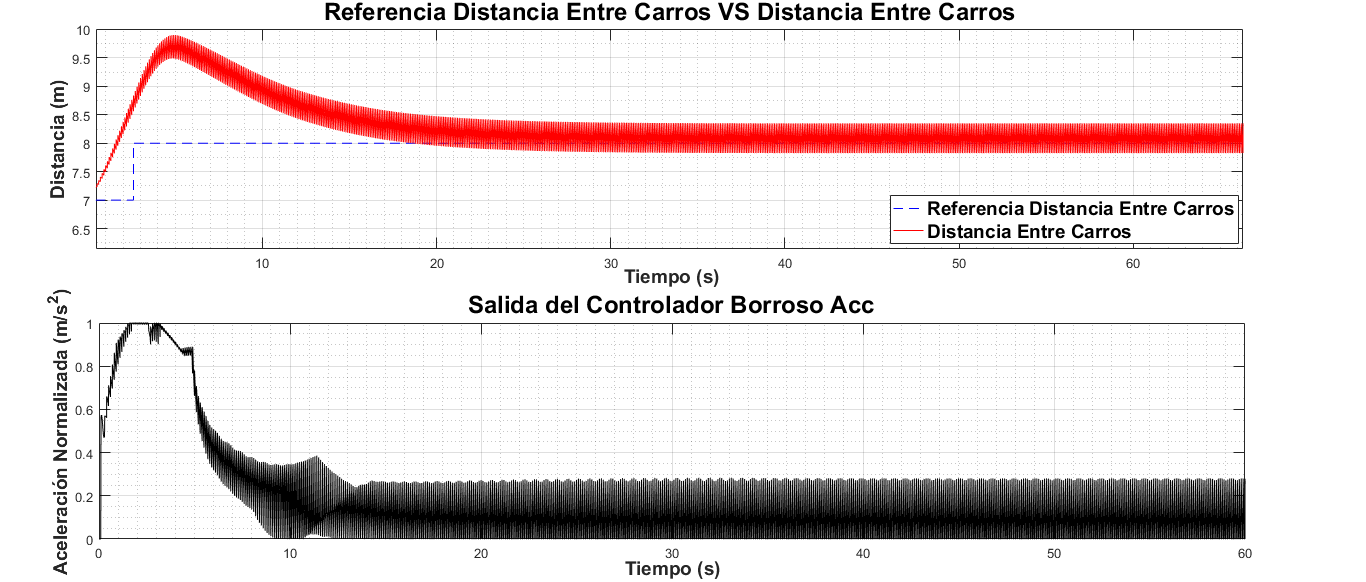
\includegraphics[scale=0.49]{Imagenes/100cv}
		\caption{Gráfica del comportamiento del controlador con una tasa de envío de 100 ms}
		\label{fig:sv100}
\end{figure}	  	  
\end{itemize}

\par Observando las figuras \ref{fig:sv1}, \ref{fig:sv5}, \ref{fig:sv10}, \ref{fig:sv15}, \ref{fig:sv25}, \ref{fig:sv50}, \ref{fig:sv100} se puede apreciar que a medida que se aumenta la tasa de envío, aumenta el ruido en el controlador, lo cual es producto de la diferencia entre el procesamiento de data a 1 ms del esquema principal del simulador, con la proveniente del bloque de recepción. Con el fin de contrastar de  mejor forma este efecto, se realizó un acercamiento a las figuras \ref{fig:sv5} y \ref{fig:sv50}, siendo este mostrado en la imagen \ref{fig:comp}:   

\begin{figure}[H]
 \centering
  \subfloat[Acercamiento de la figura \ref{fig:sv5}]{
   \label{fig:cinco}
    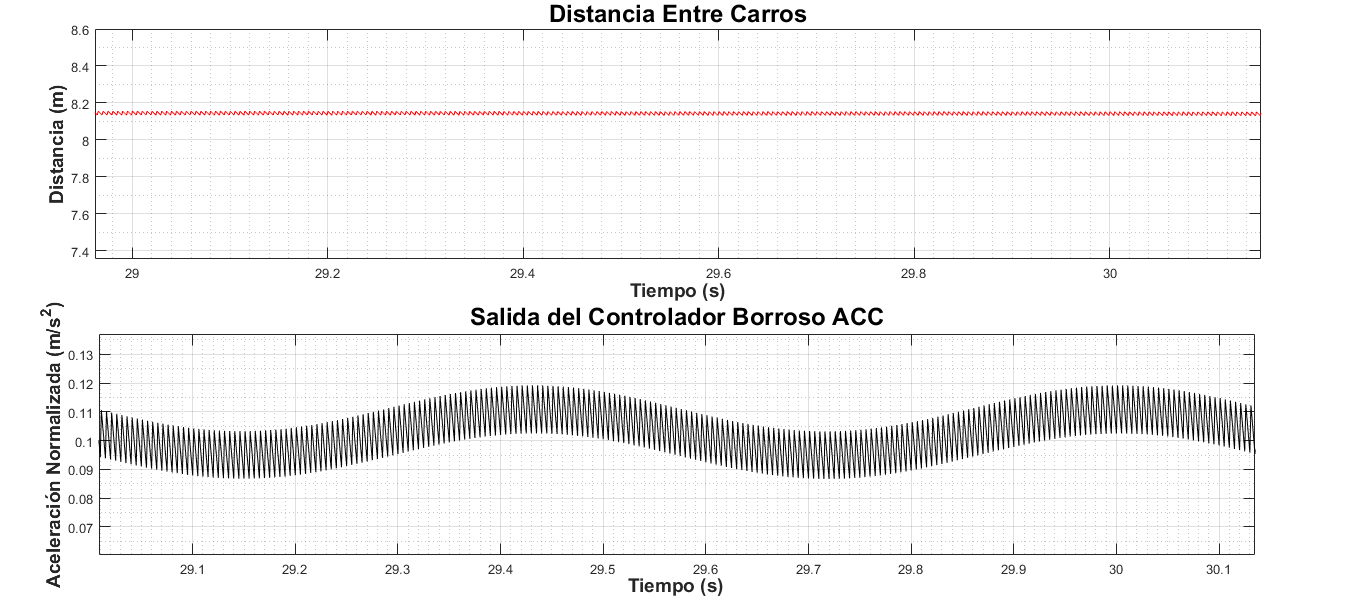
\includegraphics[scale=0.22]{Imagenes/zoom5}}
  \subfloat[Acercamiento de la figura \ref{fig:sv50}]{
   \label{fig:cincuenta}
    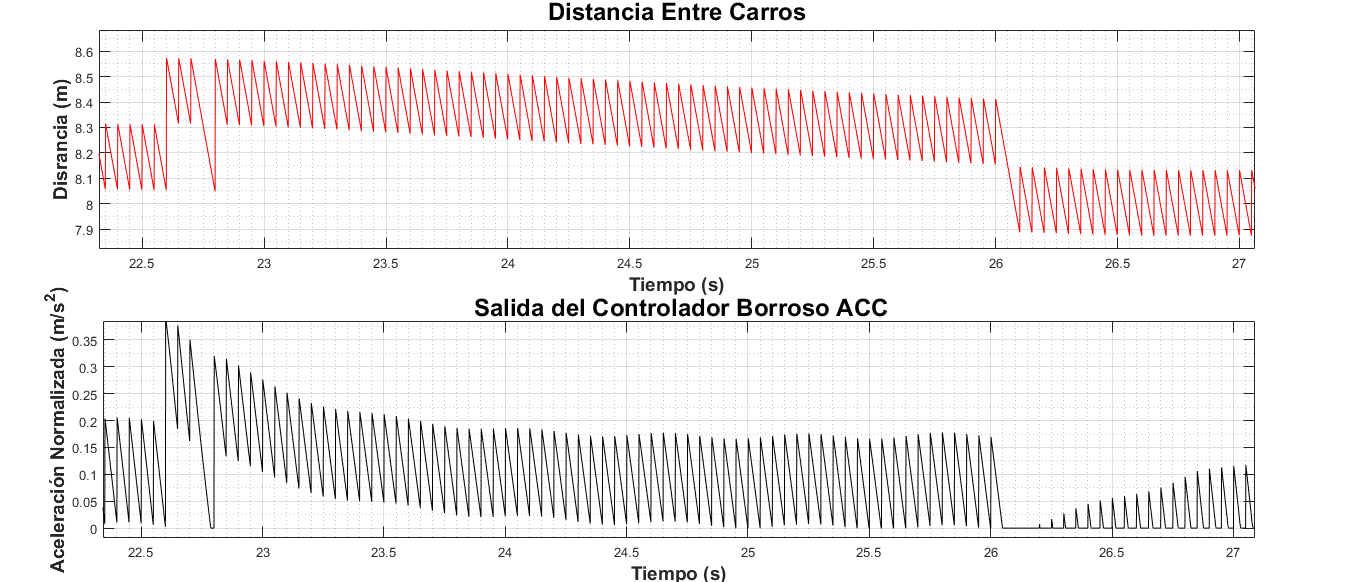
\includegraphics[scale=0.23]{Imagenes/zoom50}}\\
 \caption{Comparación entre la figuras \ref{fig:sv5} y la figura \ref{fig:sv50}}
 \label{fig:comp}
\end{figure}

\par Se puede observar en la figura \ref{fig:cinco} que efectivamente se tiene un período de 5 ms, que corresponde a la tasa de envío establecida, la cual produce una variación a la salida del controlador al estabilizarce de $ \pm 0.015$, lo que equivale a una acción del 1.5 \% sobre los actuadores, valor que posteriormente, por como están configurados el freno y el acelerador se divide a la mitad, teniendo así, un valor final del 0.75 \%, acción que puede ser considerada como despreciable. A diferencia, da la figura \ref{fig:cincuenta}, en la cual se presenta un período de 50 ms, que genera una variación de $ \pm 10 \% $, que se traduce al final en un 5 \%, dicho valor se puede ver aumentado hasta un 25 \% cuando se pierde un paquete. \\  

\par A continuación se presenta la tabla \ref{tab:tabcv}, donde se presenta la relación de menseajes totales, con mensajes perdidos. En la misma se observa que a medida de que aumenta la tasa de envío se reduce la cantidad de mensajes perdidos, así como la probabilidad de ocurrencia. De las tasas probadas se destaca la de 1 ms, la cual presenta la mayor cantidad de mensajes perdidos, efecto que se debe, a que el número de procesos manejados por el simulador al mismo tiempo, afecta de manera negativa el rendimiento de la PC, interfierendo con la recepción de data. Esto produce que se exceda con mayor frecuencia el tiempo de espera establecido sin recibir ningún paquete y de esta forma se perjudican los módulos que hacen uso de estos datos, como es apreciado en la figura \ref{fig:sv1}, donde la señal del error de la distancia tarda más tiempo (28 s) en apegarse a la referencia, a diferencia de las demás tasas (20 s). \\

\begin{table}[htbp]
  \centering
\resizebox{\textwidth}{!}{
% Table generated by Excel2LaTeX from sheet 'Hoja1'
  \begin{tabular}{|l|l|l|l|}
    \toprule
    \multicolumn{1}{|p{9.43em}|}{Tiempo de envío (ms)} & \multicolumn{1}{p{10.5em}|}{Cantidad de mensajes} & \multicolumn{1}{p{10.07em}|}{Mensajes perdidos} & \multicolumn{1}{p{8.785em}|}{\% De mensajes perdidos} \\
    \midrule
    1     & 81457 & 1909  & 2,34 \\ 
    \midrule
    5     & 16258 & 62    & 0,38 \\ 
    \midrule
    10    & 8154  & 45    & 0,55 \\ 
    \midrule
    15    & 5435  & 15    & 0,27 \\ 
    \midrule
    25    & 3260  & 13    & 0,41 \\ 
    \midrule
    50    & 1648  & 7     & 0,45 \\ 
    \midrule
    100   & 813   & 1     & 0,18 \\ 
    \bottomrule
    \end{tabular}}%
  \caption{Prueba del sistema de comunicación a distintas tasas de envío sin emplear el Visor 3D}
  \label{tab:tabsv}%
\end{table} %

\par Tomando en cuenta los resultados arrojados por las pruebas realizadas, se elijió como tasa de envío, 5 ms, ya que es la que presenta menos delay, y si bien, posee mayor perdida de paquetes que las demás tasas, no se ve afectada fuertemente, a diferencia de por ejemplo la de 25 ms, que puede generar a la salida del controlador una señal errada de más del 20 \%, tras un paquete perdido. Además, como no coincide con el tiempo de muestreo del simulador, se reducen los efectos del rendimiento del computador sobre la recepción de paquetes, mostrando así, un comportamiento más que aceptable, teniendo en cuenta las dificultadas presentadas.         

\subsubsection{Pruebas con el Visor 3D}  

A continuación, al igual que en el punto anterior, se pueden observar las gráficas del comportamiento del controlador ante las tasas de envío de 1 ms, 5 ms, 10 ms, 15 ms, 25 ms, 50 y 100 ms, pero esta vez usando el Visor 3D, el cual, además de aumentar la cantidad de procesos que tiene que ejectutar la computadora, se comunica con Simulink mediante sockets de UDP, lo que genera un mayor tráfico de paquetes, aumentando la probabilidad de que se pueda perder un paquete.   

\begin{itemize}
\item 1 ms
\begin{figure}[H]
	\centering
		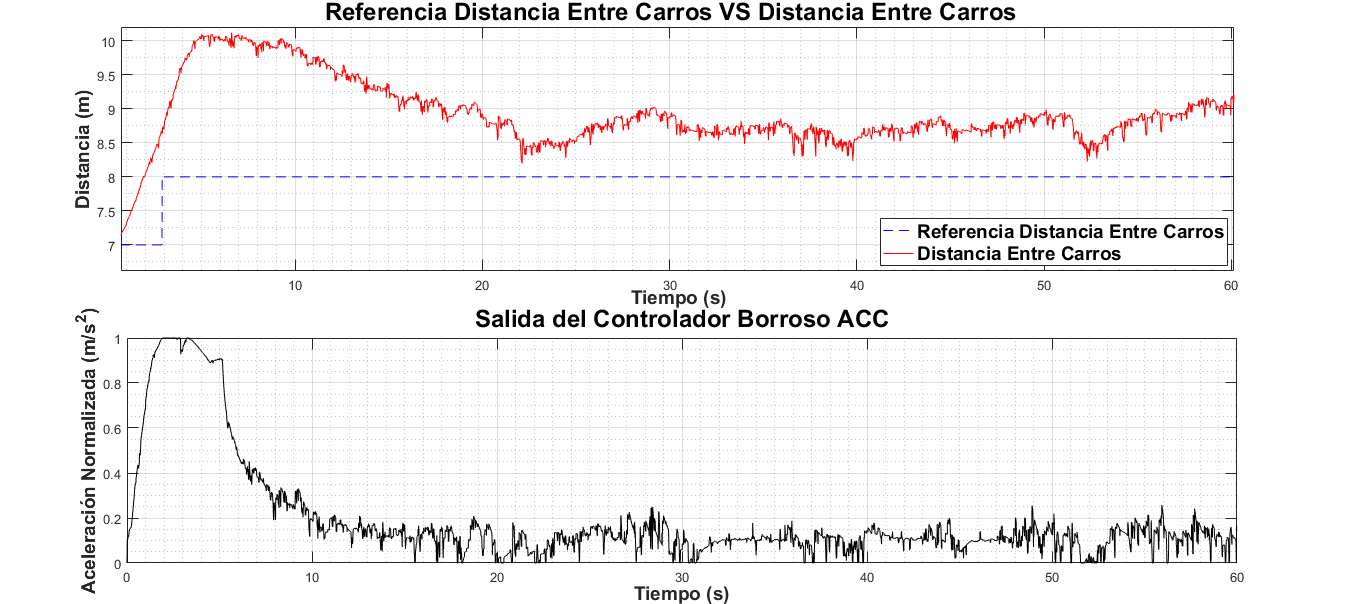
\includegraphics[scale=0.5]{Imagenes/1sv}
		\caption{Gráfica del comportamiento del controlador con una tasa de envío de 1 ms}
		\label{fig:cv1}
\end{figure}
\item 5 ms
\begin{figure}[H]
	\centering
		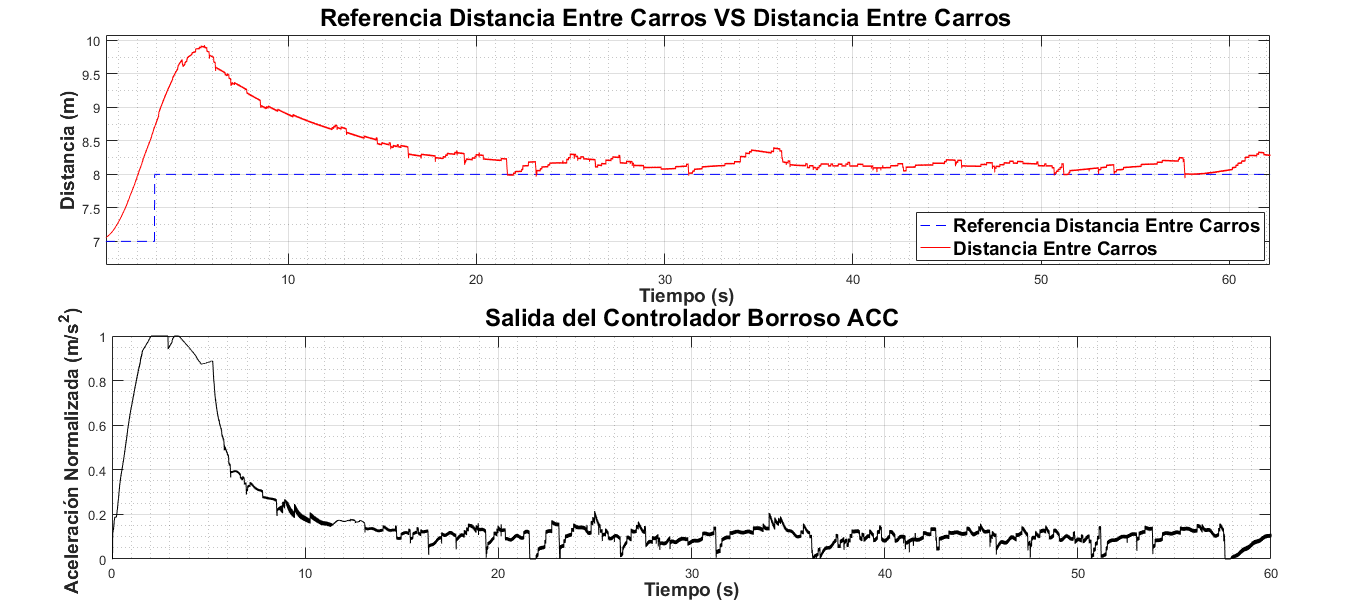
\includegraphics[scale=0.48]{Imagenes/5sv}
		\caption{Gráfica del comportamiento del controlador con una tasa de envío de 5 ms}
		\label{fig:cv5}
\end{figure}	
\item 10 ms
\begin{figure}[H]
	\centering
		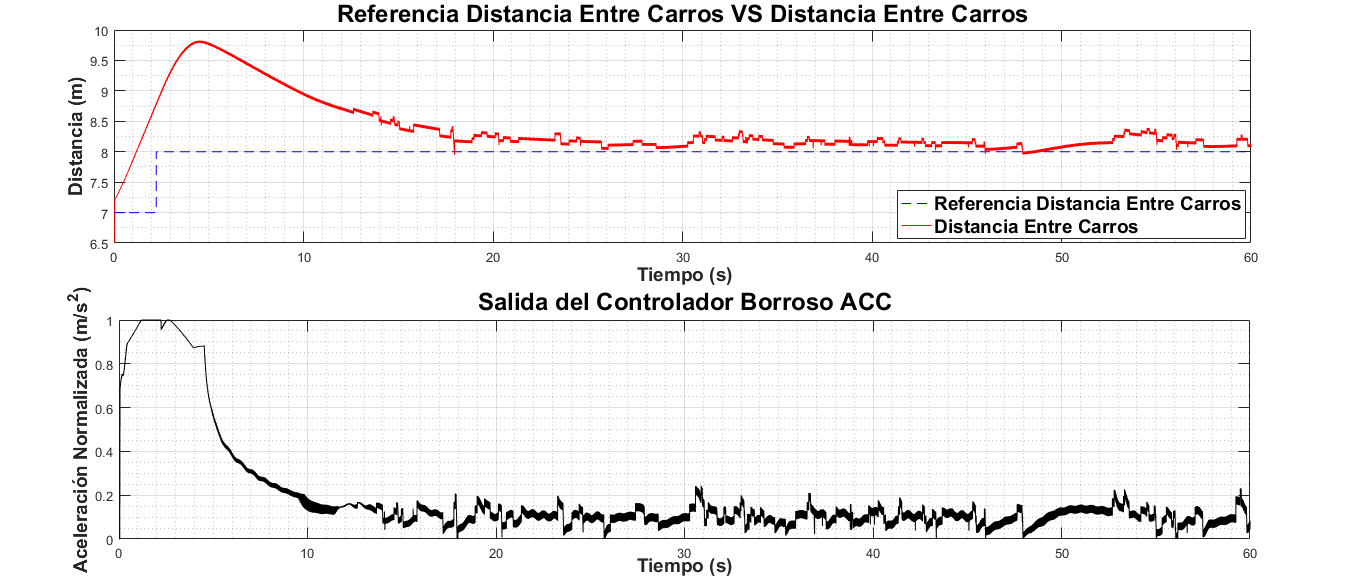
\includegraphics[scale=0.49]{Imagenes/10cv}
		\caption{Gráfica del comportamiento del controlador con una tasa de envío de 10 ms}
		\label{fig:cv10}
\end{figure}	
\item 15 ms
\begin{figure}[H]
	\centering
		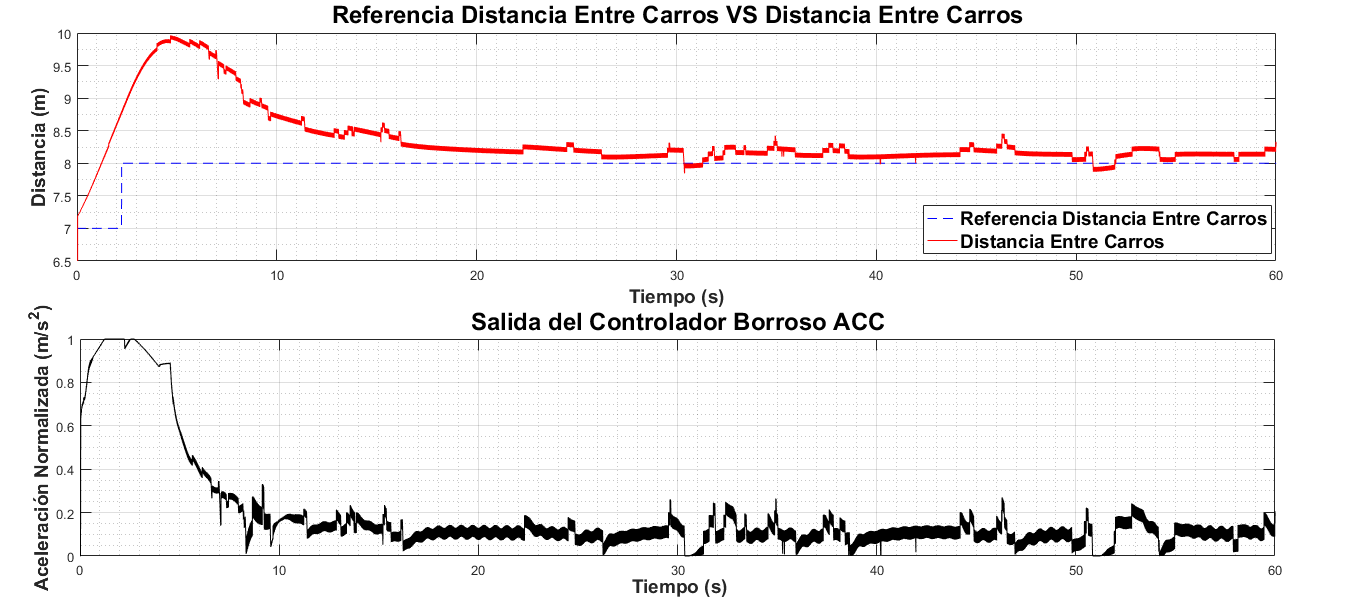
\includegraphics[scale=0.48]{Imagenes/15cv}
		\caption{Gráfica del comportamiento del controlador con una tasa de envío de 15 ms}
		\label{fig:cv15}
\end{figure}	
\item 25 ms
\begin{figure}[H]
	\centering
		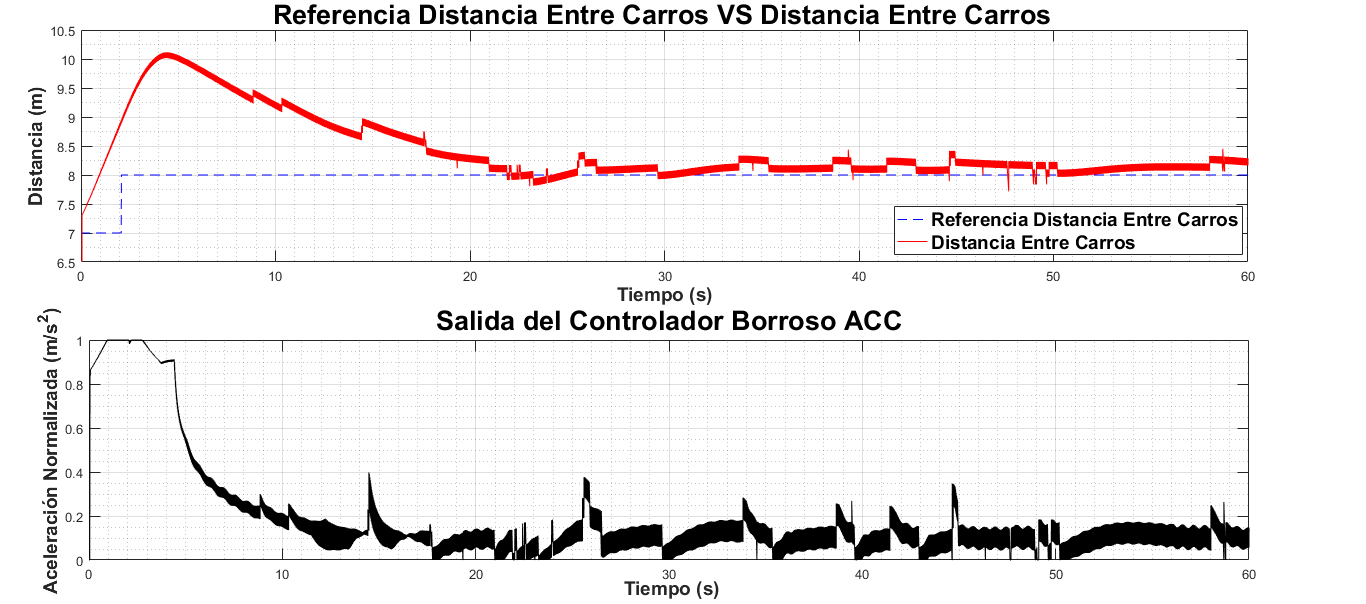
\includegraphics[scale=0.49]{Imagenes/25cv}
		\caption{Gráfica del comportamiento del controlador con una tasa de envío de 25 ms}
		\label{fig:cv25}
\end{figure}	
\item 50 ms
\begin{figure}[H]
	\centering
		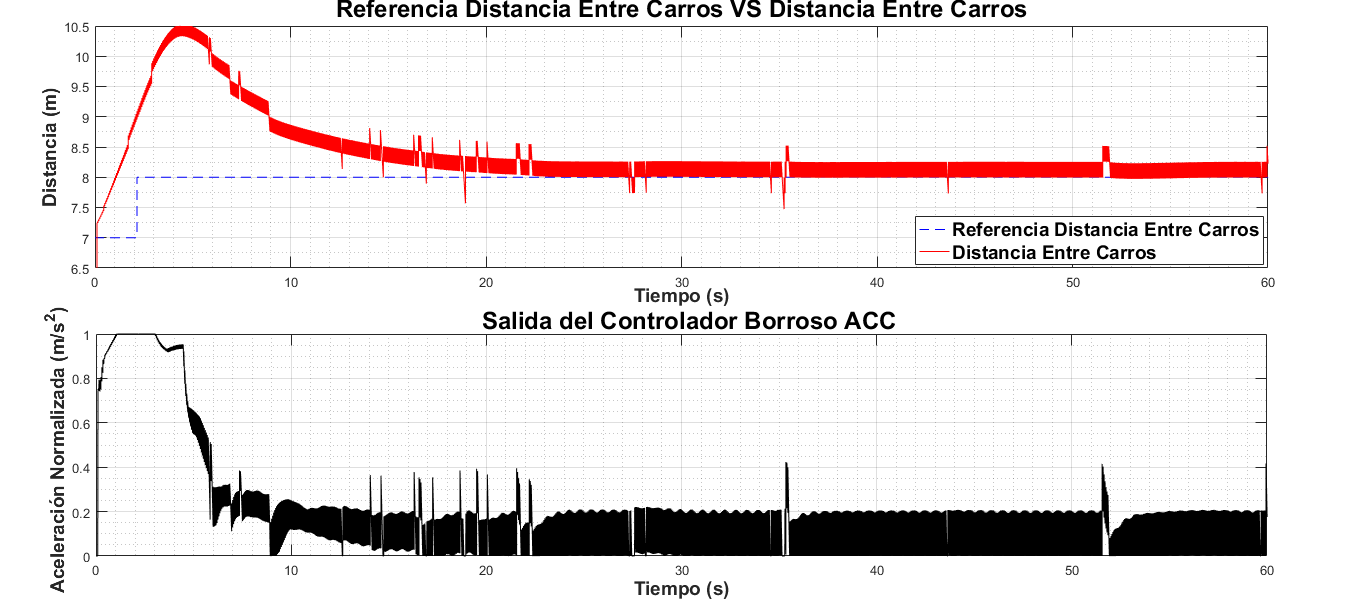
\includegraphics[scale=0.48]{Imagenes/50sv}
		\caption{Gráfica del comportamiento del controlador con una tasa de envío de 50 ms}
		\label{fig:cv50}
\end{figure}	
\item 100 ms
\begin{figure}[H]
	\centering
		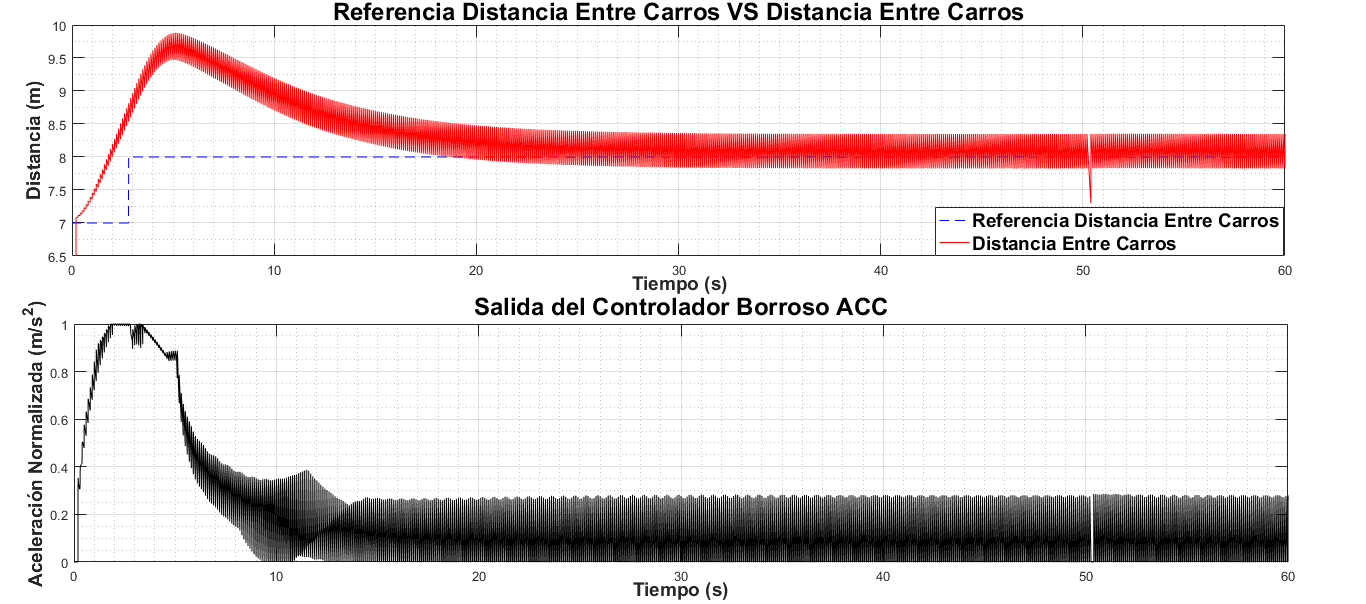
\includegraphics[scale=0.47]{Imagenes/100sv}
		\caption{Gráfica del comportamiento del controlador con una tasa de envío de 100 ms}
		\label{fig:cv100}
\end{figure}	  	  
\end{itemize}

\par Observando las figuras \ref{fig:cv1}, \ref{fig:cv5}, \ref{fig:cv10}, \ref{fig:cv15}, \ref{fig:cv25}, \ref{fig:cv50}, \ref{fig:cv100} se puede apreciar que empeoran su comportamiento con respecto a las pruebas hechas sin el visor 3D, sobre todo con la tasa de 1 ms, la cual no llega ni a apegarse a la referencia. Sin embargo la señal de la distancia si logra alcanzar la referencia, con el mismo tiempo (20 s), con las demás tasas, viendo empeorado, de esta forma solo el comportamiento del controlador, haciéndolo más suseptible ante un paquete perdido.\\      

\par De la misma forma se reportaron las estadíticas relacionadas a la cantidad de mensajes perdidos, datos que pueden ser apreciados en la tabla \ref{tab:tabcv}. 

\begin{table}[htbp]
  \centering
\resizebox{\textwidth}{!}{
% Table generated by Excel2LaTeX from sheet 'Hoja1'
    \begin{tabular}{|c|c|c|c|}
    \toprule
    \multicolumn{1}{|p{9.43em}|}{Tiempo de envío (ms)} & \multicolumn{1}{p{10.5em}|}{Cantidad de mensajes} & \multicolumn{1}{p{10.07em}|}{Mensajes perdidos} & \multicolumn{1}{p{8.785em}|}{\% De mensajes perdidos} \\
    \midrule
    1     & 81457 & 14124 & 17,34 \\
    \midrule
    5     & 16258 & 272   & 1,67 \\
    \midrule
    10    & 8154  & 132   & 1,62 \\
    \midrule
    15    & 5435  & 89    & 1,64 \\
    \midrule
    25    & 3260  & 54    & 1,64 \\
    \midrule
    50    & 1648  & 27    & 1,66 \\
    \midrule
    100   & 813   & 3     & 0,33 \\
    \bottomrule
    \end{tabular}}%
  \caption{Prueba del sistema de comunicación a distintas tasas de envío empleando el Visor 3D}
  \label{tab:tabcv}%
\end{table}%

\par De los datos obtenidos de la tabla \ref{tab:tabcv} se puede contemplar que la pérdida de paquetes es 4 veces mayor, que cuando no se usa el visor, a excepción de las tasas de 1 ms y 100 ms, siendo iguales para la útltima y 8 veces mayor para la primera, valor muy elevado, que, como se observa en la figura \ref{fig:cv1}, evita que se pueda cumplir el objetivo del controlador. Si bien la pérdida de paquetes aumentó en gran medida con respecto a las pruebas anteriores, estas probabilidades son menores al 2 \%, lo cual aún no genera un impacto lo suficientemente negativo como para no emplear alguna de estas tasas. Por lo que de la misma forma se elijío como tasa de envío la de 5 ms, ya que es la que muestra la mejor respuesta, en comparación con las demás. \\ 

\par Finalmente, se probó un último escenario, en donde la comunicación se realiza en una sola dirección, es decir un vehículo solo envía información, mientras que el otro solo recibe. Dicho escenario es el presentado en los Twizys, donde uno solo envía información (semi-automatizado), y el otro la recibe (completamente automatizado), siendo este último el encargado de realizar las maniobras. \\  

\par Para esta prueba solo se observó el comportamiento con una tasa de 1 ms, debido a que es el tiempo de muestreo del simulador, siendo 10 ms el equivalente de los vehículos. El resultado puede ser visto en la figura \ref{fig:sr}, donde en promedio, se tuvieron 361 mensajes perdidos de 81457 mensajes, representando de esta forma el 0.44 \%, disminuyendo considerablemente la cantidad de paquetes perdidos con respecto a las pruebas de las comunicaciones bidireccionales. Dicho esto se considera factible emplear una tasa de envío igual al tiempo de muestro del simulador cuando se presenta un escenario de comunicación unidireccional. 
\
\begin{figure}[H]
	\centering
		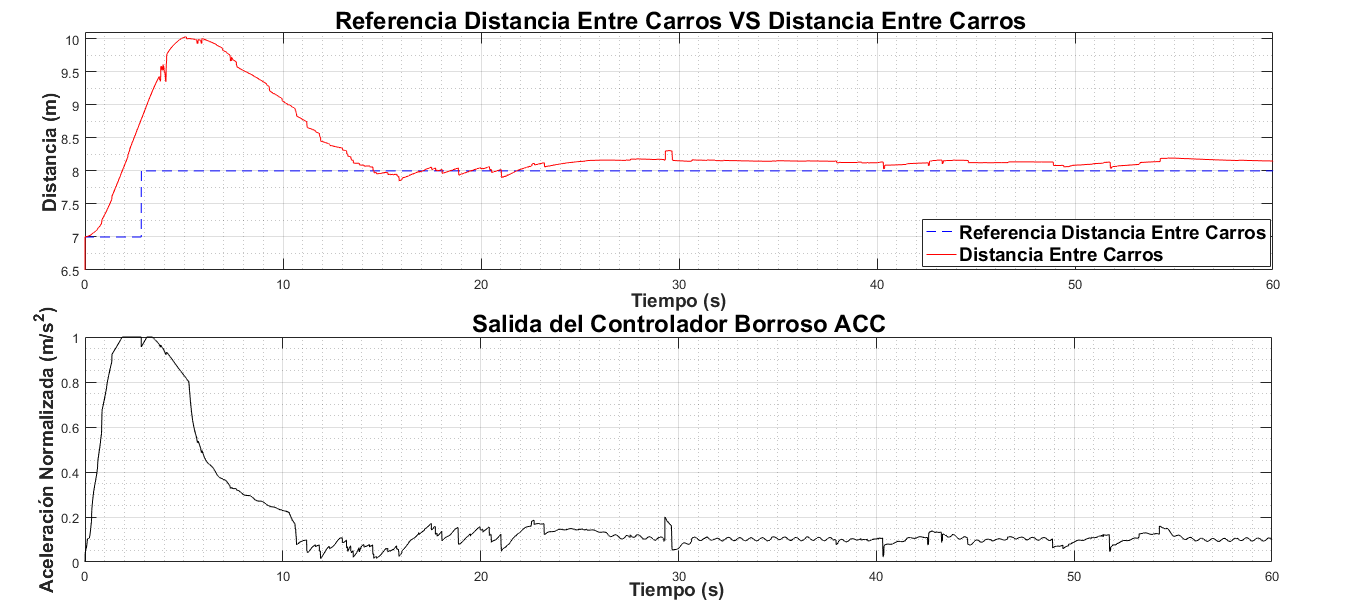
\includegraphics[scale=0.4]{Imagenes/1svc}
		\caption{Gráfica del comportamiento del controlador con una tasa de envío de 1 ms}
		\label{fig:sr}
\end{figure}	  	  

\section{Resumen}
En el capítulo 5 se presentó el sistema de comunicación implementado, argumentando el uso de dispositivos comerciales, para lo cual se realizó una exhaustiva comparación entre los protocolos de las WLAN y las VANET's. De dicha comparación se obtuvo que bajo circunstancias de bajo tráfico, donde los vehículos están ya conectados en una misma red, y se envían mensajes periódicos el sistema de comunicación comercial puede emular al vehicular.\\
\par Posteriormente, se realizó una comparación entre los protocolos de transporte UDP y TCP, que arrojó como resultado, que el más idonio es el protocolo UDP, ya que por su velocidad de transporte y no necesitar un enlace de conección fijo, puede cumplir con los requerimientos de las comunicaciones vehiculares. Luego se planteó el mensaje a usar, el cual está basado en el propuesto por la SAE.\\
\par Finalmente, se describió los bloques que conforman el sistema de comunicación implementados en Dynacar, para después observar la respuesta del sistema ante distintas tasas de envío, y las pérdidas de paquetes. De dichas pruebas se obtuvo que para ambos casos, con el Visor 3D y  sin el Visor 3D, la mejor tasa de envío es la de 5 ms, y en el caso de emplear comunicaciones unidireccionales es viable emplear una tasa igual al tiempo de muestreo del simulador, siendo 1 ms para Dynacar y 10 ms para los vehículos.      